\chapter{Top 5 Takeaways from \emph{The Social Network}}

This lecture is not a blackboard derivation in the usual sense. It is a compact entrepreneurial argument arranged as a countdown, and it moves by example, reversal, and moral extraction. We begin with a scale marker---Mark Zuckerberg as a billionaire at twenty-three---and then pass through five linked claims: persistence after failure, execution beyond ideation, disappointment as redirection, the social cost of success, and legal self-protection. Wherever we introduce a little notation below, we do so only to make the lecturer's business reasoning explicit and clean.

\section{Opening Frame: Why This Story Counts}

The lecture opens with an extraordinary outcome and only then asks what we can learn from it. The point of that opening number is not to invite a valuation model. It is simply to set the scale of the story and to justify why this film can serve as a case study in entrepreneurship.

\begin{equation}
a_{\text{Zuckerberg}} = 23
\end{equation}

This is the lecture's first numerical datum. Zuckerberg is presented as a billionaire at the age of twenty-three, and the lecturer immediately converts that fact into a program: we are to extract five practical lessons from \emph{The Social Network}. The structure matters. We are not yet being given a theory of wealth; we are being promised a guided sequence of entrepreneurial tests.

\section{Takeaway One: Persistence After the Wrong First Product}

\paragraph{Anecdote.}
The first movement of the lecture begins not with Facebook itself, but with FaceMash. The speaker uses it as the wrong first idea: crude, provocative, and costly. It brings trouble with Harvard and leads to academic probation. In that sense it is not merely incomplete; it is a failure.

\paragraph{Claim.}
From this the lecturer draws the first claim: the first business idea is often not the best one. That is already a useful correction to a romantic picture of entrepreneurship in which the winner appears fully formed at the start.

\paragraph{Mechanism.}
The reason the example matters is that failure is not treated as terminal. FaceMash does not survive, but the work does not disappear. It sits adjacent to something larger, and the lecture's pivot is that the failed attempt ultimately leads toward Facebook.

Once Facebook appears, the lecture changes register. We are no longer dealing with a single moment of invention. We are dealing with the burdens of growth. It is useful to collect those burdens in one place:
\begin{equation}
B
=
\left\{
\text{awareness},
\text{ user growth},
\text{ investor funding},
\text{ hiring},
\text{ workload},
\text{ product refinement}
\right\}
\end{equation}

This set \(B\) is not a formula taken from the lecture; it is a clean way of recording what the lecturer lists in prose. The point is that persistence is not vague determination. It is the ability to continue under a sequence of changing constraints. A business first struggles to exist, then struggles to spread, then struggles to finance its own expansion, then struggles to staff itself, and finally struggles to refine the product while the founder is carrying a punishing workload.

So the lecturer's first lesson has a definite structure. We do not say merely that hard work is good. We say that entrepreneurial work is prolonged contact with obstacles, and persistence is the capacity to keep working while the form of the obstacle changes.

\section{Takeaway Two: Execution Beats Possession of the Idea}

\paragraph{Anecdote.}
The lecture then turns to the Winklevoss twins and ConnectU. They too want a social platform. They too have ambition. But the lecturer insists that the key difficulty is not wanting such a platform. It is building one.

\paragraph{Claim.}
This gives us the second lesson: it is not about who has the idea; it is about who can execute on the idea. In the lecture's rhythm, this is a refinement of the first takeaway. Persistence alone is not enough; persistence must attach to construction.

\begin{definition}
Let \(I\) denote an idea, let \(E\) denote execution capacity---the relevant skill, organization, and team ability to build---and let \(O\) denote a realized operating outcome.
\end{definition}

With that notation, the lecturer's point may be written in deliberately spare form as
\begin{equation}
I \neq O,
\qquad
I + E \longrightarrow O.
\end{equation}

This is only shorthand, but it helps. An idea is not yet a business. An idea plus execution can become one.

The lecture closes this example with a hard institutional number:
\begin{equation}
S_{\text{Winklevoss settlement}} = \$65\,\text{million}.
\end{equation}

The settlement matters, but only in a limited way. It is not the proof that ideas are decisive. It is the coda that shows how idea-ownership disputes can persist even after execution has already decided who built the dominant platform. The lecturer's emphasis stays where it began: a great idea without the skill or team to realize it remains only an idea.

\section{Takeaway Three: Not Getting What One Wants Can Be a Blessing}

\paragraph{Anecdote.}
The lecture's third movement begins with the film's breakup scene: Mark is presented as being broken up with, returning home angry, and then creating FaceMash. But here the speaker pauses and qualifies the story. He says this was actually false in historical terms. That pause is essential. It creates the most natural conceptual tension in the lecture.

\subsection{Question \& Answer}

\paragraph{Question.}
If the movie scene is historically false, why keep it in the lecture at all?

\paragraph{Answer.}
Because the lecturer is no longer treating the scene as court evidence. He is treating it as a thematic model. The literal causal chain may be wrong, but the entrepreneurial pattern remains useful: not getting what one wants can force a redirection, and that redirection may open the path to something larger. The lecture is careful here. It does not say the film scene is true. It says the theme is good.

\paragraph{Mechanism.}
Once that distinction is made, the lecturer turns to a broader pattern:
\begin{equation}
\text{blocked outcome}
\;\longrightarrow\;
\text{disruption or failure}
\;\longrightarrow\;
\text{new attempt}
\;\longrightarrow\;
\text{larger opportunity}.
\end{equation}

This is the cleaned-up logical spine of the third takeaway. It is not an empirical law and not a guaranteed update rule. It is a way of stating what the speaker means by ``when one door closes, another one opens.''

It is helpful to draw the structure in a narrow schematic.

\begin{figure}
\centering
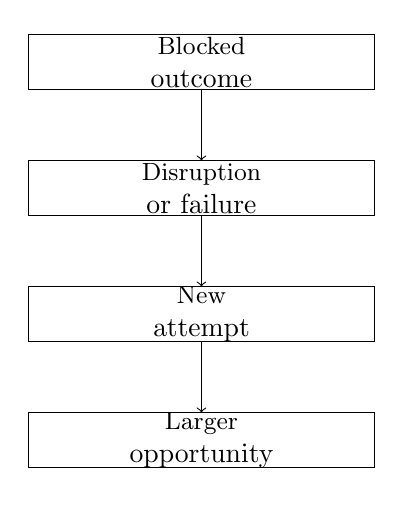
\begin{tikzpicture}[x=1cm,y=1cm]
\draw (-2.2,0.35) rectangle (2.2,-0.35);
\node[align=center] at (0,0) {\small Blocked\\outcome};

\draw (-2.2,-1.25) rectangle (2.2,-1.95);
\node[align=center] at (0,-1.6) {\small Disruption\\or failure};

\draw (-2.2,-2.85) rectangle (2.2,-3.55);
\node[align=center] at (0,-3.2) {\small New\\attempt};

\draw (-2.2,-4.45) rectangle (2.2,-5.15);
\node[align=center] at (0,-4.8) {\small Larger\\opportunity};

\draw[->] (0,-0.35) -- (0,-1.25);
\draw[->] (0,-1.95) -- (0,-2.85);
\draw[->] (0,-3.55) -- (0,-4.45);
\end{tikzpicture}
\end{figure}

The lecturer then replaces the movie anecdote with his own evidence. He says that failed businesses in his own life led him to the opportunity he is working on now, namely School of Hard Knocks. That move is important. The lecture does not remain trapped inside the film. It uses the film to raise a pattern and then re-grounds the pattern in direct entrepreneurial testimony.

\section{Takeaway Four: Scale Produces Opposition}

\paragraph{Claim.}
The fourth lesson is introduced with a deliberate rhetorical beat: ``you can't'' repeated several times before the thought is completed. The completed claim is that one cannot be ultra successful without making a few enemies.

\paragraph{Mechanism.}
What the lecturer means is not mysterious. Success at scale expands the surface on which other people can resist, resent, compete with, or simply dislike what we are doing. The lecture gives Mark Zuckerberg as the example, but the point is quickly generalized: on any serious journey there will be naysayers, non-believers, and people who do not care about us.

Here the lecture makes another important turn. It does not answer hostility with a fantasy of universal persuasion. Instead it narrows the stabilizing variables to two: the inner circle and self-belief. In other words, once scale creates opposition, the entrepreneurial task is not to eliminate every enemy. It is to remain oriented while conflict becomes part of the environment.

This section is easy to flatten into a slogan about ``haters.'' The lecture is doing something slightly more precise than that. It is saying that social resistance is not accidental noise at the edge of success. It is one of the ordinary prices of building something large.

\section{Takeaway Five: Shares, Dilution, and the Need to Lawyer Up}

\paragraph{Anecdote.}
The lecture ends with its hardest institutional warning. Eduardo Saverin, in the film, has his shares diluted. The speaker emphasizes negligence, blind signing, and a failure to understand what was happening. Whatever the exact historical details may be, the lecture's practical point is sharp: brilliance and friendship do not remove the need for legal care.

To make the business logic precise, let us introduce the one formal definition the lecture clearly invites.

\begin{definition}
If owner \(i\) holds \(s_i\) shares out of a total of \(S\) shares outstanding, define the owner's fraction of the company by
\begin{equation}
f_i = \frac{s_i}{S}.
\end{equation}
After a transaction or restructuring, we write the new quantities as
\begin{equation}
f_i' = \frac{s_i'}{S'}.
\end{equation}
\end{definition}

The lecturer's warning about dilution can then be expressed cleanly.

\begin{proposition}
If an owner's own share count stays fixed while the total share count rises, then the owner's ownership fraction falls. In symbols,
\begin{equation}
s_i' = s_i,
\qquad
S' > S
\quad \Longrightarrow \quad
f_i' < f_i.
\end{equation}
\end{proposition}

\begin{proof}
If \(s_i' = s_i\), then
\[
f_i' = \frac{s_i}{S'}.
\]
Since \(S' > S > 0\), dividing the same positive numerator by the larger denominator produces the smaller fraction:
\[
\frac{s_i}{S'} < \frac{s_i}{S}.
\]
But \(\frac{s_i}{S} = f_i\). Hence \(f_i' < f_i\).
\end{proof}

This is the clean algebraic content behind the lecture's cautionary story. We are not reconstructing the exact Facebook cap table. We are simply writing down the mechanism that the lecturer wants us to understand.

A small numerical example makes the point immediate. Suppose, purely for illustration, that owner \(i\) has
\begin{align}
s_i &= 30,
&
S &= 100,
&
f_i &= 0.30.
\end{align}
If the owner's own shares do not rise but the total count doubles, then
\begin{align}
s_i' &= 30,
&
S' &= 200,
&
f_i' &= 0.15.
\end{align}
The owner still has shares, but the owner's fraction of the company has been cut in half.

\begin{remark}
The lecture supports the qualitative fact of dilution, not the exact legal mechanics. The example above is therefore illustrative. It should not be read as a claim about the actual historical percentages in Facebook.
\end{remark}

From here the lecturer turns immediately to advice. The mathematical fraction is the formal shadow of a practical warning. Before one signs documents involving shares, ownership, or partnership rights, one must slow down and do due diligence.

\begin{itemize}
\item Understand what is being signed and what quantities may change.
\item Separate friendship from ownership structure.
\item Treat partnership documents as binding business instruments, not as gestures of trust.
\item Get legal counsel before signing away rights that affect shares, control, or future upside.
\end{itemize}

The lecture's final takeaway is therefore more than ``be careful.'' It is that entrepreneurial optimism must be matched by institutional literacy. A company can be built by vision and labor, but ownership can still be altered by paper.

\section{Summary}

The lecture moves in a clear sequence, and it is worth keeping that sequence intact.

\begin{enumerate}
\item An early failure may be the wrong product, not the end of the journey.
\item An idea is not yet a business; execution is what turns concept into outcome.
\item A blocked desire or failed path may redirect us toward a larger opportunity.
\item Success at scale brings enemies, and so self-belief and a trusted inner circle matter.
\item Ownership requires legal care, because shares and control can change through agreements that are not fully understood.
\end{enumerate}

Taken together, these five takeaways form a practical entrepreneurial chain. We begin with the false start, we pass to execution, we reinterpret disappointment, we accept the social cost of scale, and we end with the legal protection of ownership. The speaker closes by recommending the film; the notes close by observing why it works for him as a teaching device. It is not a perfect historical record, but it is a useful sequence of entrepreneurial test cases.